\documentclass[10pt,landscape,a4paper]{article}
\usepackage[utf8]{inputenc}
\usepackage{listings}
\usepackage{color}
\usepackage[ngerman]{babel}
\usepackage[T1]{fontenc}
%\usepackage[LY1,T1]{fontenc}
%\usepackage{frutigernext}
%\usepackage[lf,minionint]{MinionPro}
\usepackage{tikz}
\usetikzlibrary{shapes,positioning,arrows,fit,calc,graphs,graphs.standard}
\usepackage[nosf]{kpfonts}
\usepackage[t1]{sourcesanspro}
\usepackage{multicol}
\usepackage{wrapfig}
\usepackage[top=5mm,bottom=5mm,left=5mm,right=5mm]{geometry}
\usepackage[framemethod=tikz]{mdframed}
\usepackage{microtype}
\usepackage{pdfpages}
\usepackage{titlesec}


\usepackage{graphicx}

\titleformat*{\section}{\large\bfseries}
\titleformat*{\subsection}{\normalsize\bfseries}
\titleformat*{\subsubsection}{\small\bfseries}

\titlespacing*{\section}
{0pt}{1.5ex plus 0.2ex}{1.5ex plus .2ex}
\titlespacing*{\subsection}
{0pt}{1.5ex plus .2ex}{1.5ex plus .2ex}
\titlespacing*{\subsubsection}
{0pt}{1.5ex plus .2ex}{1.5ex plus .2ex}

\graphicspath{ {./images} }

\newtheorem{definition}{Definition}[section]

\definecolor{dkgreen}{rgb}{0,0.6,0}
\definecolor{gray}{rgb}{0.5,0.5,0.5}
\definecolor{mauve}{rgb}{0.58,0,0.82}

\lstset{frame=tb,
  language=Java,
  aboveskip=3mm,
  belowskip=3mm,
  showstringspaces=false,
  columns=flexible,
  basicstyle={\small\ttfamily},
  numbers=none,
  numberstyle=\tiny\color{gray},
  keywordstyle=\color{blue},
  commentstyle=\color{dkgreen},
  stringstyle=\color{mauve},
  breaklines=true,
  breakatwhitespace=true,
  tabsize=3,
  basicstyle = \footnotesize
}

\let\bar\overline



\begin{document}
%\footnotesize
\footnotesize
\begin{multicols*}{4}
\section{Time Complexity}
{Master's theorem for $T(n) = aT(\frac{n}{b}) + f(n)$ where $a \geq 1$ and $b > 1$} \\
Let $c_{crit} = log_b(a)$ and if $f(n) = \theta(n^c)$
\begin{enumerate}
    \item {If $c < c_{crit}$ then $T(n) = \theta(n^{c_{crit}})$} 
    \item {If $c = c_{crit}$ then $T(n) = \theta(n^clog(n))$} 
    \item {If $c > c_{crit}$ then $T(n) = \theta(f(n))$} 
    \item {If $f(n) = \theta(n^{c_{crit}}log^k(n))$, then $T(n) = \theta(n^{c_{crit}}log^{k+1}(n))$} 

\end{enumerate}

\section{Sorting}
\subsection{Bubblesort}
\textbf{Time complexity: $\Omega({n})$ $\theta(n^2)$ $O(n^2)$} \\
Invariant: At the end of iteration \texttt{j}, the biggest \texttt{j} items are correctly sorted in the final \texttt{j} positions of the array.

\subsection{SelectionSort}
\textbf{Time complexity: $\Omega({n^2})$ $\theta(n^2)$ $O(n^2)$} \\
Invariant: At the end of iteration \texttt{j}: the smallest \texttt{j} items are correctly sorted in the first \texttt{j} positions of the array.

\subsection{InsertionSort}
\textbf{Time complexity: $\Omega({n})$ $\theta(n^2)$ $O(n^2)$} \\
Invariant: At the end of iteration \texttt{j}: the first \texttt{j} items of the array are sorted in order.

% \begin{lstlisting}
%    for (x = 1 to arr.len):
% 	j = x - 1
% 	store = arr[x]
% 	while(j >= 0 && arr[j] > store):
% 		arr[j + 1] = arr [j]
% 		j--
% 	arr[j+1] = store
% \end{lstlisting}

\subsection{QuickSort}
\textbf{Time complexity: $\Omega({nlog(n)})$ $\theta(nlog(n))$ $O(n^2)$ $O(nlog(n))$ (for paranoid QuickSort)}  \\
Invariant: For every \texttt{i < low}: \texttt{B[i] < pivot} and for every \texttt{j > high}: \texttt{B[j] > pivot}.
Duplicates: Use three-way partition to store duplicates.

\subsection{MergeSort}
\textbf{Time complexity: $\Omega({nlog(n)})$ $\theta(nlog(n))$ $O(nlog(n))$} \\
Invariant: At the end of each loop, the subarrays are sorted.

\subsection{QuickSelect}
\textbf{Time complexity: $\Omega(n)$ $\theta(n)$ $O(n^2)$} \\ 
Invariant: For every \texttt{i < low}: \texttt{B[i] < pivot} and for every \texttt{j > high}: \texttt{B[j] > pivot}.


%\subsection{TopoSort}
%\textbf{Time complexity: $O(V+E)$.}


% Trees section
\section{Trees}

\subsection{Binary Search Tree (BST)}
Only has 2 children per node. Left child is smaller than parent. Right child is larger than parent. \\
Operations: $O(log(n))$ / $O(n)$ (balanced)

\subsection{AVL Tree}
Maximum height between two children tree is 1. \\
Operations: $O(log(n))$ \\
% \textbf{Left Rotation:} \\
% 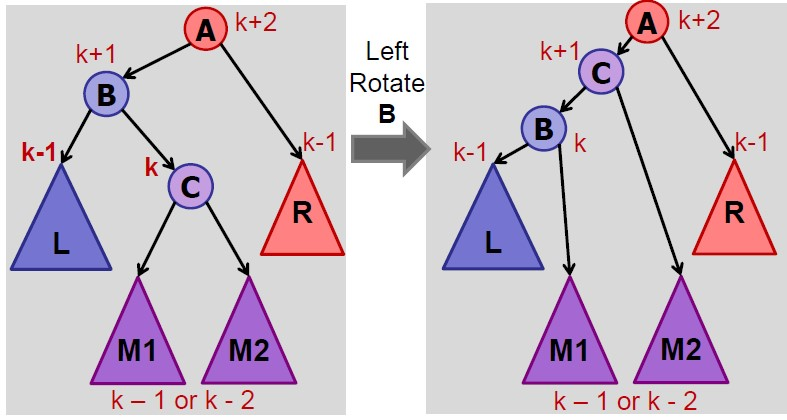
\includegraphics[width = 6cm]{left-rotate} \\
% \textbf{Right Rotation:} \\
% 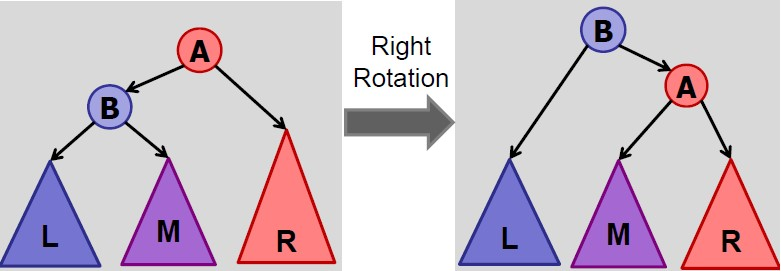
\includegraphics[width = 6cm]{right-rotate} \\
\textbf{Insertion Max Rotations:} 2 \\
\textbf{Deletion Max Rotations:} $log(n)$ \\
\textbf{Invariant}: \texttt{|height(u) - height(v)| < 2} if \texttt{v} and \texttt{u} are sibling nodes. \texttt{|height(u) - height(v)| > 0} if \texttt{u} is the parent node of \texttt{v}.
% \columnbreak
\subsection{Order Statistics (Rank finding)}
AVL Tree augmented with a \texttt{weight} property in each node. \\
Updating weights on rotate: $O(1)$ 
% \begin{lstlisting}
%     rank = weight(node.right) + 1
%     while(node != null && node.parent != null):
% 	    if (node.parent.left == node):
% 		    rank += weight(node.parent.right) + 1
% 		    node = node.parent

%     FindRanks(currentRank, node, targetRank):
% 	    check = currentRank + weight(node.left) + 1
% 	    if (check == targetRank):
% 		    return node
% 	    elif (check < targetRank):
% 		    return FindRanks(currentRank, node.right, targetRank)
% 	    else:
% 		    return FindRanks(currentRank, node.left, targetRank)
% \end{lstlisting}

\subsection{Interval Trees}
Store the maximum value of entire subtree under a node as a parameter. Update \texttt{max} during rotations by taking \texttt{Math.max} of all children under the two nodes being swapped. \\
\textbf{Time complexity: $O(log(n))$} \\
% \begin{lstlisting}
%     interval-search(x)
%         c = root;
%         while (c != null and x is not in c.interval) do
%             if (c.left == null) then
%                 c = c.right;
%             else if (x > c.left.max) then
%                 c = c.right;
%             else c = c.left;
%                 return c.interval;
% \end{lstlisting}

\subsection{1D Range Finding}
All leaves hold the value, each internal node \texttt{v} stores the \texttt{MAX} of any leaf in the left sub-tree. \\
% \begin{center}
%     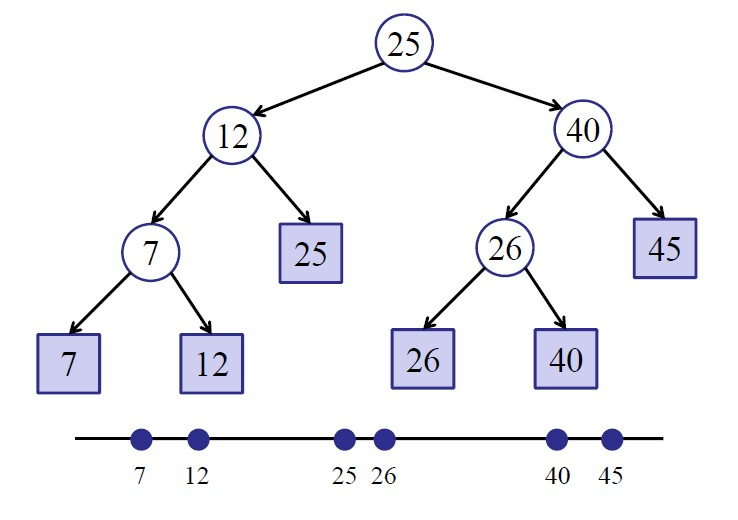
\includegraphics[width = 4cm]{1d-range}
% \end{center}
\textbf{Operations}: \\
\begin{tabular}{p{2cm} p{3.5cm}}
    \verb!findSplit!        & Finds the node to start searching. \\
    \verb!traverseLeft!     & Traverse the left subtree after findSplit. \\
    \verb!traverseRight!    & Traverse the right subtree after findSplit.\\
\end{tabular}\\
\textbf{Complexity}: \\
\begin{tabular}{p{2cm} p{3.5cm}}    
    \verb!Query!    & $O(k + log(n))$ \\
    \verb!Build!    & $O(nlog(n))$ \\
    \verb!Space!    & $O(n)$ \\
\end{tabular}
\subsection{(a, b) trees}
An (a, b) tree has a bound of $2 \le a \le \frac{b+1}{2}$.\\\\
\textbf{Rule 1:}\\\\
\begin{tabular}{c|c|c|c|c}
    Node Type   &   \multicolumn{2}{|c|}{\#Keys} &  \multicolumn{2}{|c}{\#Children} \\
    {}          &   Min     &   Max            &    Min     &   Max \\
    \hline
    Root        &   1       &   b - 1           &   2       &   b   \\
    \hline
    Internal    &   a - 1   &   b - 1           &   a       &   b   \\
    \hline
    Leaf        &   a - 1   &   b - 1           &   0       &   0   \\
\end{tabular} \\\\
\textbf{Rule 2:} A \textbf{non-leaf node} must have one more child than its number of keys. \\
\textbf{Rule 3:} All \textbf{leaf nodes} must be at the same depth (from the root). \\
\begin{tabular}{p{0.6cm} p{5.4cm}}
    \verb!search!   & Traverse from the root node and binary search the node array. ($O(log(n))$).\\
    \verb!insert!   & Traverse from the root to find point of insertion. Split if needed ($O(log(n))$).  \\
    \verb!delete!   & Traverse from the root to find node and delete. Sacrifice/merge/split if needed ($O(log(n))$). \\
    \verb!split!    & Find the median element in the node array and sacrifice to the parent. The split halves are now the child of the promoted node. \\
    \verb!merge!    & Merges two siblings. Delete the parent and add the parent to the keylist of one child. Merge the two children. \\
    \verb!share!    & Merge and split combined. \\
\end{tabular}

\section{Hashing}

\subsection{Hashing with Chaining}
If a current bucket is occupied, add to the linked list in the bucket. 
\begin{itemize}
    \item \textbf{Insert:} $O(1 + cost(f))$ 
    \item \textbf{Search/Delete:} $O(n + cost(f))$ where $n$ is the number of nodes. 
    \item Expected Number of items per bucket = $\frac{n}{m}$. 
    \item Under Simple Uniform Hashing Assumption (every key is likedly to be mapped to every permutation), $E(\text{search}) = O(1)$.
    \item Can still add items when $m == n$ and search efficiently.
\end{itemize}

\subsection{Hashing with Open Addressing}
If the current bucket is full, find the next available bucket (Linear Probing).
\begin{itemize}
    \item \textbf{Insert/Delete/Search:} $O(1)$ if $\alpha < 1$ where $\alpha = \frac{n}{m}$ where $n$ is the \#items and $m$ is \#buckets. 
    \item When deleting a key, replace the bucket with \texttt{DELETED}. Functions will probe past \texttt{DELETED}. 
    \item Clusters of size $\Theta(log(n))$ form when table is $\frac{1}{4}$ full. Caching of arrays make this fast.
    \item Unable to insert and search efficiently when $m == n$.
    \item Expected cost of operation is $\le \frac{1}{1-a}$.
\end{itemize}

\subsection{Double Hashing}
Two ordinary hash functions $f(k)$ and $g(k)$ with new hash function:
\begin{equation*}
    h(k, i) = f(k) + i \cdot g(k) \; mod m
\end{equation*}
$g(k)$ must be relatively prime to $m$ for $h(k, i)$ to hit all buckets.

\subsection{Hashcode}
\begin{tabular}{p{1.5cm} p{4.5cm}}
    \verb!Integer!      &   The int value itself. \\
    \verb!Long!         &   Split the long into 32 bits, XOR. \\
    \verb!String!       &   Iterate through each char, sum the value with an offset. \\
\end{tabular}

\subsection{Resizing}
If $(n == m)$, then $m = 2m$ and if $(n < \frac{m}{4})$, then $m = \frac{m}{2}$. \\
\begin{definition}
    Operation has amortized cost $T(n)$ if for every integer $k$, the cost of $k$ operations is $\le k T(N)$.
\end{definition}

\subsection{HashSet}
\begin{itemize}
    \item Stores a bit instead of key.
    \item $P(\text{false positive})$ = $1 - (1-\frac{1}{n})^n \approx 1 - (\frac{1}{e})^{\frac{n}{m}}$.
\end{itemize}

\subsection{Bloom Filter}
\begin{itemize}
    \item Use 2 hash functions $f(k)$ and $g(k)$. Both buckets must return \texttt{True} for a positive match.
    \item $P(\text{false positive})$ = $(1 - \frac{1}{e}^{\frac{2n}{n}})^2$.
    \item $P(\text{bit is 0}) = (1 - \frac{1}{m})^{kn} \approx e^{-kn/m}$.
    \item $P(\text{collision at 1 spot}) = 1 - e^{-kn/m}$.
    \item $P(\text{collision at 1 spot}) = (1 - e^{-kn/m})^k$

\end{itemize}

\section{Graphs}
% \begin{definition}
    % A graph consists of at least a node, and can consist of edges that connect nodes in the graph.
% \end{definition}
% \begin{definition}
    % A connected graph has all nodes connected by a path.
% \end{definition}
% \begin{definition}
    % The degree of a node is the number of adjacent edges on that node.
% \end{definition}
% \begin{definition}
    % The degree of a graph is the maximum number of adjacent edges in the graph.
% \end{definition}
% \begin{definition}
    % Diameter is the maximum distance between two nodes following the shortest path.
% \end{definition}
% \begin{definition}
    % Star graph has all nodes connected to a central node.
% \end{definition}
% \begin{definition}
    % Clique is a complete graph with diameter $1$ and degree $n-1$.
% \end{definition}
\begin{definition}
    A cycle is a connected graph with a loop. It has a diameter $\frac{n}{2}$ or $\frac{n}{2}-1$ and degree $2$.
\end{definition}
\begin{definition}
    A bipartite graph is a graph with nodes divided into two sets. There are no edges between nodes of the same set.
\end{definition}
\begin{definition}
    \textbf{Cayley's Formula:} The number of possible MSTs of a complete graph is $V^{V-2}$.
\end{definition}

\subsection{Representation}
\begin{itemize}
    \item Adjacency List. Each node has a linked list of edges to other nodes. ($O(V+E)$ memory).
    \item Adjacency Matrix. 2D array that stores path from a node to another. ($O(V^2)$ memory).
\end{itemize}

\subsection{Traversal}
\begin{itemize}
    \item BFS. Use a queue to explore neighbours level by level.
    \item DFS. Use a stack to explore the maximum depth, then neighbours.
\end{itemize}

\subsection{Directed Acyclic Graph}
A topological sorted graph can find shortest paths in $O(E)$ by walking through the graph once.
\subsubsection{Post-order DFS}
\begin{itemize}
    \item Use post-order DFS to add nodes to the set.
    \item Time Complexity: $O(V+E)$.
\end{itemize}

\subsubsection{Kahn's Algorithm}
\begin{itemize}
    \item Maintain a set of nodes with no incoming edges. Remove edges and add them to the set when a node has no incoming edge. 
    \item Time Complexity: $O(E log(V))$ or $O(E +V)$.
\end{itemize}

\subsection{Shortest Paths}
\subsubsection{Bellman Ford}
\begin{itemize}
    \item Relax all edges $V$ times. Can detect negative weight cycles. 
    \item Time Complexity: $O(EV)$ (Can optimise to terminate early when no weight changes detected). 
    \item Negative weight cycles can be detected with $|V| + 1$ iterations. To label all negative weight cycles, run for $2|V|$. 
\end{itemize}

\subsubsection{Dijkstra's}
\begin{itemize}
    \item Relax shortest edge using a priority queue.
    \item Time Complexity: $O(Elog(V))$ (Assumes PQ operations are $log(v)$).
    \item Each edge is relaxed once and each node is added to the priority queue once.
\end{itemize}


\section{Heaps}
Binary heap stores inserts nodes from left to right and ensures the maximum height is $O(floor(log(n)))$. \\
\begin{tabular}{p{2cm} p{4cm}}
   \verb!insert! & $O(log(n))$ \\
   \verb!delete! & Swap with min element and \texttt{bubbleDown} min element. $O(log(n))$ \\
   \verb!decreaseKey! & $O(log(n))$ \\
   \verb!extractMax!    & $O(log(n))$ \\
\end{tabular}\\
For a lookup array (swap positions when we bubble):
\begin{tabular}{p{2cm} p{4cm}}
    \verb!leftChild!    &   $2x+1$ \\
    \verb!rightChild!   &   $2x+2$  \\
    \verb!parent!       &   $floor((x-1)/2)$ 
\end{tabular}

\subsection{Heapify}
Bubble from leaf upwards, recursively ensured that subtrees are heaps.
\begin{lstlisting}
    for (int i = n - 1; i > =0; i--):
        bubbleDown(i, A) // O(logn)
\end{lstlisting}
\textbf{Time Complexity:}
\begin{align*}
    \sum_{h=0}^{h = log(n)} \frac{n}{2^h} O(h) 
    % \le& cn(\frac{1}{2} +\frac{2}{2^2} + \frac{3}{2^3} + \frac{4}{2^4} + ...) \\
    % \le& cn(\frac{1/2}{1-1/2}^2) \\
    \le& 2 \cdot O(n)
\end{align*}

\subsection{HeapSort}
Extract the max and put it at the back of the HeapArray.
\begin{lstlisting}
    for (int i = n -1; i >= 0; i--):
        A[i] = extractMax(A);
\end{lstlisting}
\begin{itemize}
    \item \textbf{Time Complexity:} $O(nlog(n))$.
    \item Unstable, inplace, faster than MS, slower than QS, deterministic (always $O(nlog(n))$).
\end{itemize}

\section{UFDS}

\subsection{QuickFind}
\textbf{Time Complexity:} Find: $O(1)$ Union: $O(n)$
\begin{tabular}{p{1cm} p{5.5cm}}
    \verb!find! &   Check the int array if two items have the same id. \\
    \verb!union!    &   \texttt{union(p, q)} change all items with id of \texttt{p} to id of \texttt{q}.
\end{tabular}

\subsection{QuickUnion}
\textbf{Time Complexity:} Find: $O(n)$ Union: $(n)$
\begin{tabular}{p{1cm} p{5.5cm}}
    \verb!find! &   Check the ADT if two items have the same parent id. \\
    \verb!union!    &   \texttt{union(p, q)} change parent of \texttt{q} to id of \texttt{parent(p)}.
\end{tabular}
QuickUnion(1, 4): \\
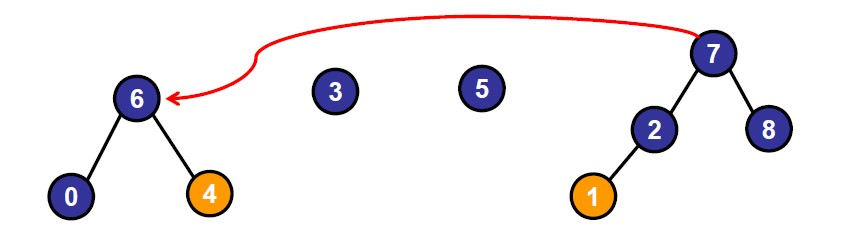
\includegraphics[width=7cm]{quickunion}

\subsubsection{Weighted Union}
\textbf{Time Complexity:} Find: $O(log(n))$ Union: $(log(n))$ \\
Connect the parent in order of size to ensure the height of tree is $O(log(n))$.

\subsubsection{Path Compression}
\textbf{Time Complexity:} $O(n + m\alpha(m, n))$. \\
When \texttt{find} is called, compress each traversed parent to the found root.

\section{MST}
\textbf{Properties:}
\begin{enumerate}
    \item No cycles
    \item If you cut an MST, both pieces are MSTs.
    \item For every cycle, the max weight edge is NOT in.
    \item For every cut, the min weight is in the MST.
\end{enumerate}

\subsection{Prim's Algorithm}
\textbf{Time Complexity:} $O(E log(V))$. \\
Queue all nodes in a PQ. Decrease key for every adjacent edge of dequeued node.

\subsection{Kruskal's Algorithm}
\textbf{Time Complexity:} $O(E log(V))$. \\
Sort all edges. Use UFDS, add edges if the two nodes are not in the same set.

\subsection{Boruvka's Algorithm}
\textbf{Time Complexity:} $O(E log(V))$. \\
\textbf{Step 1:} Add all minimum adjacent edges. \\
\textbf{Step 2:} Add minimum edge out of each connected component. Repeat till 1 connected component left.

\subsection{Variants}
For all edges having weights from \textbf{\{1..10\}}.
\subsubsection{Kruskal}
\textbf{Time Complexity:} $O(\alpha E)$.
\begin{enumerate}
    \item Put all edges array of linked lists.
    \item Iterate through all edges and check to union or not.
\end{enumerate}

\subsubsection{Prim's}
\textbf{Time Complexity:} $O(V + E) \approx O(E)$.
\begin{enumerate}
    \item Use an array of size 10 as PQ, each slot holding a linked list.
    \item \texttt{decreaseKey} moves node from 1 linked list to another. ($O(E)$).
\end{enumerate}

\subsubsection{Directed MST}
Only works for a \textbf{DAG with one "root"}. \\
Walk through the graph prioritising weights, maintaining \texttt{visited[]}. 

\subsubsection{Steiner (2-approx)}
\begin{enumerate}
    \item For every required vertex, calculate the shortest path.
    \item Construct new graph with the required nodes.
    \item Run MST and map new edges to original graph.
\end{enumerate}



\section{Dynamic Programming}

\subsection{Longest Increasing Subsequence}
\textbf{Time Complexity:} $O(n^2)$.
\begin{enumerate}
    \item Start from the last item.
    \item Find the maximum outgoing edge and add 1 and store.
    \item Recurse until the array is iterated through
\end{enumerate}

\subsection{Lazy Prize Collection}
\textbf{Time Complexity:} $O(kE)$.
\begin{enumerate}
    \item Subproblem: \texttt{P[v,k]} = maximum prize you can collect starting at v, taking \texttt{k} steps. 
    \item \texttt{P[v,k] = MAX\{ P[$w_1$, k-1] + w(v, $w_1$), P[$w_2$, k-1] + w(v, $w_2$), $\dots$ \}} where \texttt{v.nbrlist() = \{$w_1$, $w_2$, $w_3$, $\dots$ \}}
\end{enumerate}

\subsection{Vertex Cover}
Set of nodes $C$ where every edge is adjacent to at least one node in $C$.
\begin{enumerate}
    \item \texttt{S[v,0]} = size of vertex cover in subtree at \texttt{v} if \texttt{v} is NOT covered.
    \subitem \texttt{S[v,0]} = \texttt{S[$w_1$, 1] + S[$w_2$, 1] + $\dots$}
    \item \texttt{S[v,1]} = size of vertex cover in subtree at \texttt{v} if \texttt{v} is covered.
    \subitem \texttt{S[v,1]} = \texttt{1 + min(S[$w_1$, 0], S[$w_1$, 1] + min(S[$w_2$, 0], S[$w_2$, 1]) + $\dots$}
\end{enumerate}

\subsection{APSP (Floyd Warshall)}
\textbf{Time Complexity:} $O(V^3)$.
\begin{enumerate}
    \item \texttt{S[v,w,P]} = shortest path from \texttt{v} to \texttt{w} that only uses intermediate nodes in set $P$.
    \item Use a 2D array and solve for $S$ as we add more nodes into set $P$.
    \item \texttt{S[v,w,$P_i$] = min (S[v,w,$P_{i-1}$], S[v,i,$P_{i-1}$] + S[i,w,$P_{i-1}$])}
\end{enumerate}

\subsubsection{Path Reconstruction}
Reconstruct the shortest path by storing a \texttt{predecessor[]} and update whenever we update a node's shortest path.

\subsubsection{Transitive Closure}
Instead of finding the distance, we want to know if there exist a path. \\
Change to: \texttt{S[v,w,$P_i$] = \textbf{OR} (S[v,w,$P_{i-1}$], S[v,i,$P_{i-1}$] \textbf{AND} S[i,w,$P_{i-1}$])}


\section{Recitation BS}

\subsection{MET}
Iterate through 3 dimensions (ins, del, rep) to achieve the destination string. Since it is a DAG, topo-sort and run SSSP.

\subsection{Leftist Heaps}
\textbf{Property:} For every node that has two children $L$, $R$, \texttt{rightRank(L) >= righRank(R)}.\\
\begin{tabular}{p{1.5cm}p{5cm}}
    \verb!insert! $O(log(n))$   &   Insert down the right spine. If \texttt{Pr(curr) > Pr(orig)}, swap the two nodes. Insert when a node with no right child is found. Update \texttt{rightRank} as the recursion unrolls. \\
    \verb!merge! $O(log(n))$   &   Walk down the right spine and compare the root. If the merging root is of higher priority, swap the subtree and recursively merge on the subtree. Walk down and check if any swaps are required for the LEFTIST property. \\
    \verb!extractMax! $O(log(n))$   &   Remove the root and call \texttt{merge} on the left and right subtree. \\
    \verb!delete! $O(log(n))$   &   Delete the node and swap if LEFTIST property is violated. Walk up and update \texttt{rightRank}. \\
    \verb!updateKey! $O(log(n))$ &  Call delete and insert.

    
\end{tabular}

\subsection{Indirection}
Group continuous sequence in an array to a node, and have a pointer to the next element.


\subsection{Minimax}
\begin{enumerate}
    \item Use Binary Search.
    \item Use Floyd Warshall/APSP.
    \item Use MST then BFS/DFS.
    \item Use Lowest Common Ancestor search tree.
\end{enumerate}
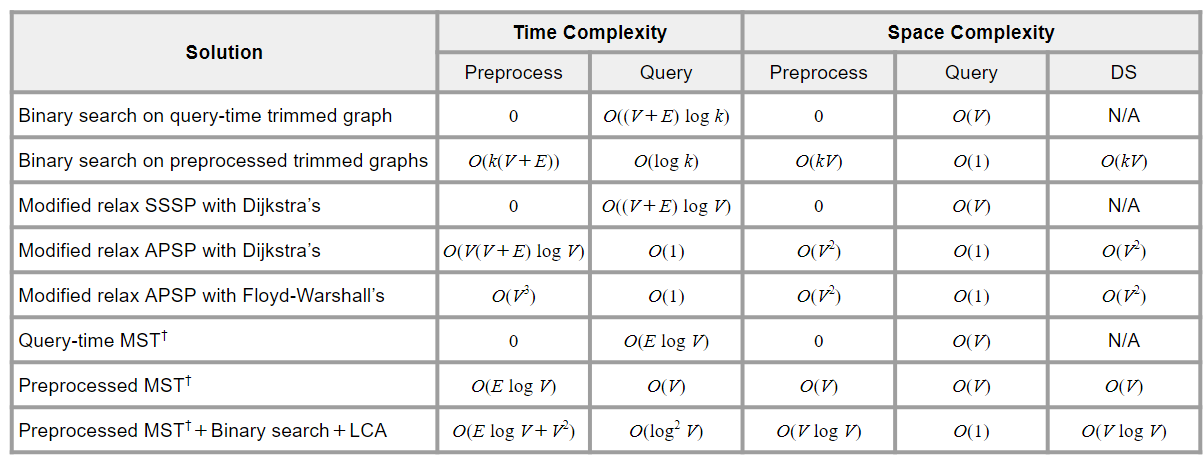
\includegraphics[width=7cm]{minimax}


\end{multicols*}
\end{document}